\documentclass[../main/main]{subfiles}

\setcounter{chapter}{4}
%\setcounter{page}{1}
\begin{document}
\chapter{実験条件}

\section{多目的ベンチマーク問題}
\quad 本項では,本研究の数値実験で用いる24個のベンチマーク問題の構造について述べる.
\Tabref{benchmark}に本研究に用いるベンチマーク問題をその性質とともに示す.

\begin{table}[htbp]
\fontsize{9.5pt}{9.5pt} \selectfont
\tabcolsep = 1pt
\centering
\caption{本研究で取り扱うベンチマーク問題}
\vspace{0.1cm}
\label{benchmark}
\begin{tabular}{cccc||cccc}
\hline 
Problem & Obj. &Var. & Con. & Separability & Modality & Bias & Geometry \\
\hline 
DTLZ2 & M & N & - & separable & uni & - & concave\\
DTLZ3 & M & N & - & separable & multi & - & concave\\
DTLZ4 & M & N & - & separable & uni & \checkmark & concave\\
DTLZ7 & M & N & - & separable & uni & - & concave, disconnected\\
WFG2 & M & N & - & non-separable & multi & - & convex, disconnected\\
WFG4 & M & N & - & separable & multi & - & concave\\
WFG6 & M & N & - & non-separable & uni & - & concave\\
WFG7 & M & N & - & separable & uni & \checkmark & concave\\
WFG8 & M & N & - & non-separable & multi & - & concave\\
UF2 & 2 & N & - & non-separable & multi & - & convex\\
UF9& 3 & N & - & non-separable & multi & - & linear, disconnected\\
CF2 & 2 & N & 1 & non-separable & multi & - & convex, disconnected\\
CF7 & 2 & N & 2 & non-separable & multi & - & convex\\
C1DTLZ3 & M & N & 1 & separable & multi & - & concave\\
C2DTLZ2convex & M & N & 1 & separable & uni & - & convex, disconnected\\
C3DTLZ1 & M & N & M & separable & multi & - & convex(feasible surface is PF)\\
Car Side Impact & 3 & 7 & 10 & & & uncertain &\\
Welded Beam Design& 2 & 4 & 4 & & & uncertain &\\
Modified DTLZ2 & M & N & - & separable & uni & - & concave\\
Modified DTLZ3 & M & N & - & separable & multi & - & concave\\
Modified DTLZ4 & M & N & - & separable & uni & \checkmark & concave\\
Multi DTLZ2 & M & N & - & separable & uni & - & concave\\
Multi DTLZ3 & M & N & - & separable & multi & - & concave\\
Multi DTLZ4 & M & N & - & separable & uni & \checkmark  & concave\\
\hline
\end{tabular}
\\
{\scriptsize Obj. is the number of objectives; Var. is the number of variables; Con. is the number of constraints.}\\
{\scriptsize $M$ is the user predefined number of objectives; $N$ is the user predefined number of variables.}\\
{\scriptsize - indicates no value or no characteristic; \checkmark indicates that the problem has the characteristic.}\\
{\scriptsize The Car Side Impact and Welded Beam Design problems have uncertain characterisics because of engineering problems.}
\end{table}


\Tabref{benchmark}において,Problemは多目的ベンチマーク問題の名称を示している.
また,Obj.,Var.,Con.,はそれぞれ各多目的ベンチマーク問題の目的関数の数,設計変数の数,制約条件の数を示す.
MやNで示される目的関数の数,設計変数の数は,ユーザが任意に設定することができる.

Separabilityは各設計変数が相関関係にあるか否かを示している.
separableは相関関係なし,non-separableは相関関係ありを示す.
separableな問題な場合,各設計変数の最適値は一意に定まる.
一方で,non-separableな問題な場合,各設計変数の最適値は一意に定まらず,他の設計変数の値に応じて変化する.
したがって,non-separableな問題のほうがseparableな問題に比べ,最適化が難しい傾向にある.

Modalityは局所最適解があるか否かを示している.
uniは単峰性の性質を持つ問題を示しており,局所最適解は存在せず大域的最適解のみが存在する問題である.
一方で,multiは多峰性の性質を持つ問題を示しており,局所最適解を有する問題である.
多峰性の性質を持つ問題は局所最適解を持つため,大域的最適解に収束しづらく,単峰性の性質を持つ問題と比較し,一般的に最適化が難しい傾向にある.

Biasは目的関数空間において,解が偏りを持って生成されてしまう性質を有するか否かを示している.
$\checkmark$で示される問題は,目的関数空間に解が射影される際,強い非線形性によって,解が局所的に集中しやすく,目的関数空間全体を覆うような多様性のある解を生成することが難しい問題である.
したがって,Biasがある問題のほうが解の多様性を維持した最適解を得ることが難しい傾向にある.

Geometryは真のパレート最適解の形状を示している.
最適化手法によっては,真のパレート最適解の形状により得手不得手があるため,様々な形状の多目的ベンチマーク問題で性能を評価する必要がある.

次節以降でそれぞれの問題の構造を詳しく述べる.

\subsection{DTLZ問題}
DTLZ問題\cite{}は2002年にDebらによって提案された多目的ベンチマーク問題である.
大きな特徴として,1)目的関数の数と設計変数の数をユーザ自身が決定できる,2)設計変数が目的関数空間内の位置を決定する変数と目的関数空間内での原点からの距離を決定する変数に分離されている,ことが挙げられる.
本論文では,これらの変数をそれぞれ位置変数,距離変数と呼ぶこととする.
本研究ではDTLZ2,3,4を用いる.

\subsubsection{DTLZ2}
DTLZ2は\Eqref{dtlz2}で表される多目的ベンチマーク問題である.
DTLZ2は局所解を持たない単峰性の多目的問題であり,真のパレート最適開集合は半径1の超球面上に分布する.
目的関数の数を$M$,設計変数の数を$n \geq M$とした場合,設計変数$x_1,\cdots,x_{M-1}$は位置変数となり,残りの設計変数$x_M,\cdots,x_n$は距離変数となる.
各目的関数$f_m(m=1, \cdots ,M)$の係数$(1+g(\bm{x}_M))$が原点からの距離に相当する.
したがって,DTLZ2の真のパレート最適解を得るためには,位置変数$x_1,\cdots,x_{M-1}$が一様に広がっており,$g(\bm{x}_M)$が$0$,すなわちすべての距離変数$x_M,\cdots,x_n$が$0.5$となる必要がある.

\begin{eqnarray} 
\left.
\begin{array}{ll}
Min. \quad f_{1} (\bm{x}) = (1+g(\bm{x}_{M}))\cos(x_{1}\pi/2)  \cdots  \cos(x_{M-2}\pi/2)\cos(x_{M-1}\pi/2),\\
Min. \quad f_{2} (\bm{x}) = (1+g(\bm{x}_{M}))\cos(x_{1}\pi/2)  \cdots  \cos(x_{M-2}\pi/2)\sin(x_{M-1}\pi/2), \\
Min. \quad f_{3} (\bm{x}) = (1+g(\bm{x}_{M}))\cos(x_{1}\pi/2)  \cdots  \sin(x_{M-2}\pi/2), \\
     \  \  \ $\vdots$    \qquad     \qquad      \qquad     \qquad \vdots \\
Min. \quad f_{M}(\bm{x}) = (1+g(\bm{x}_{M}))\sin(x_{1}\pi/2)\\
with \quad g(\bm{x}_{M}) = \sum_{x_i \in \bm{x}_M} (x_i - 0.5)^2  \\
   \qquad    \qquad    \qquad  \quad      0 \le x_{i} \le 1,  for \ i = 1, 2, \ldots, n. \\
   \qquad    \qquad    \qquad  \quad        \bm x = (x_1,x_2, \ldots, x_n)\\
   \qquad    \qquad    \qquad  \quad        \bm{x}_M = (x_M,x_{M+1}, \ldots, x_n)
   \label{dtlz2} 
\end{array}
\right\}
\end{eqnarray}

\subsubsection{DTLZ3}
DTLZ3は \Eqref{dtlz3} で表される多目的ベンチマーク問題である.
DTLZ3は局所最適解を持つ多峰性の多目的問題であり,パレート最適解は半径1の超球面上に分布する.
DTLZ2と同様に,設計変数$x_1,\cdots,x_{M-1}$は位置変数,設計変数$x_M,\cdots,x_n$は距離変数となり,各目的関数$f_m$の係数$(1+g(\bm{x}_M))$が原点からの距離に相当する.
DTLZ2と異なる点は,$g(\bm{x}_M)$が振動する点である.
$g(\bm{x}_M)$が振動するため局所最適解を複数個持つこととなる.
例として図  \ref{fig:dtlz3_gx}に$M=3$,$n=38$,$x_3=x_4= \cdots =x_n$の時の距離変数による$g(\bm{x_M})$の推移を示す.

図 \ref{fig:dtlz3_gx}より$x_3=x_4= \cdots =x_n=0.5$の時,$g(\bm{x_M})=0$の最小値を取ることが分かる.
したがって,DTLZ3の真のパレート最適解を得るためには,位置変数$x_1,\cdots,x_{M-1}$が一様に広がっており,$g(\bm{x}_M)$が$0$,すなわちすべての距離変数$x_M,\cdots,x_n$が$0.5$となる必要がある.


\begin{eqnarray} 
\left.
\begin{array}{ll}
Min. \quad f_{1}  (\bm{x}) = (1+g(\bm{x}_{M}))\cos(x_{1}\pi/2)  \cdots  \cos(x_{M-2}\pi/2)\cos(x_{M-1}\pi/2),\\
Min. \quad f_{2} (\bm{x}) = (1+g(\bm{x}_{M}))\cos(x_{1}\pi/2)  \cdots  \cos(x_{M-2}\pi/2)\sin(x_{M-1}\pi/2), \\
Min. \quad f_{3} (\bm{x}) = (1+g(\bm{x}_{M}))\cos(x_{1}\pi/2)  \cdots  \sin(x_{M-2}\pi/2), \\
     \  \  \ $\vdots$    \qquad     \qquad      \qquad     \qquad \vdots \\
Min. \quad f_{M}(\bm{x}) = (1+g(\bm{x}_{M}))\sin(x_{1}\pi/2)\\
with\ g(\bm{x}_{M}) = 100[|\bm{x}_{M}| 
 +\sum_{x_i \in \bm{x}_M} (x_i - 0.5)^2  - \cos(20\pi(x_i-0.5)) ] \\
   \qquad    \qquad   \qquad  \quad  0 \le x_{i} \le 1,  for\ i = 1, 2, \ldots, n. \\
      \qquad    \qquad    \qquad  \quad        \bm x = (x_1,x_2, \ldots, x_n)\\
   \qquad    \qquad    \qquad  \quad        \bm{x}_M = (x_M,x_{M+1}, \ldots, x_n)
   \label{dtlz3} 
\end{array}
\right\}
\end{eqnarray}

\begin{figure}[htbp]
\begin{center}
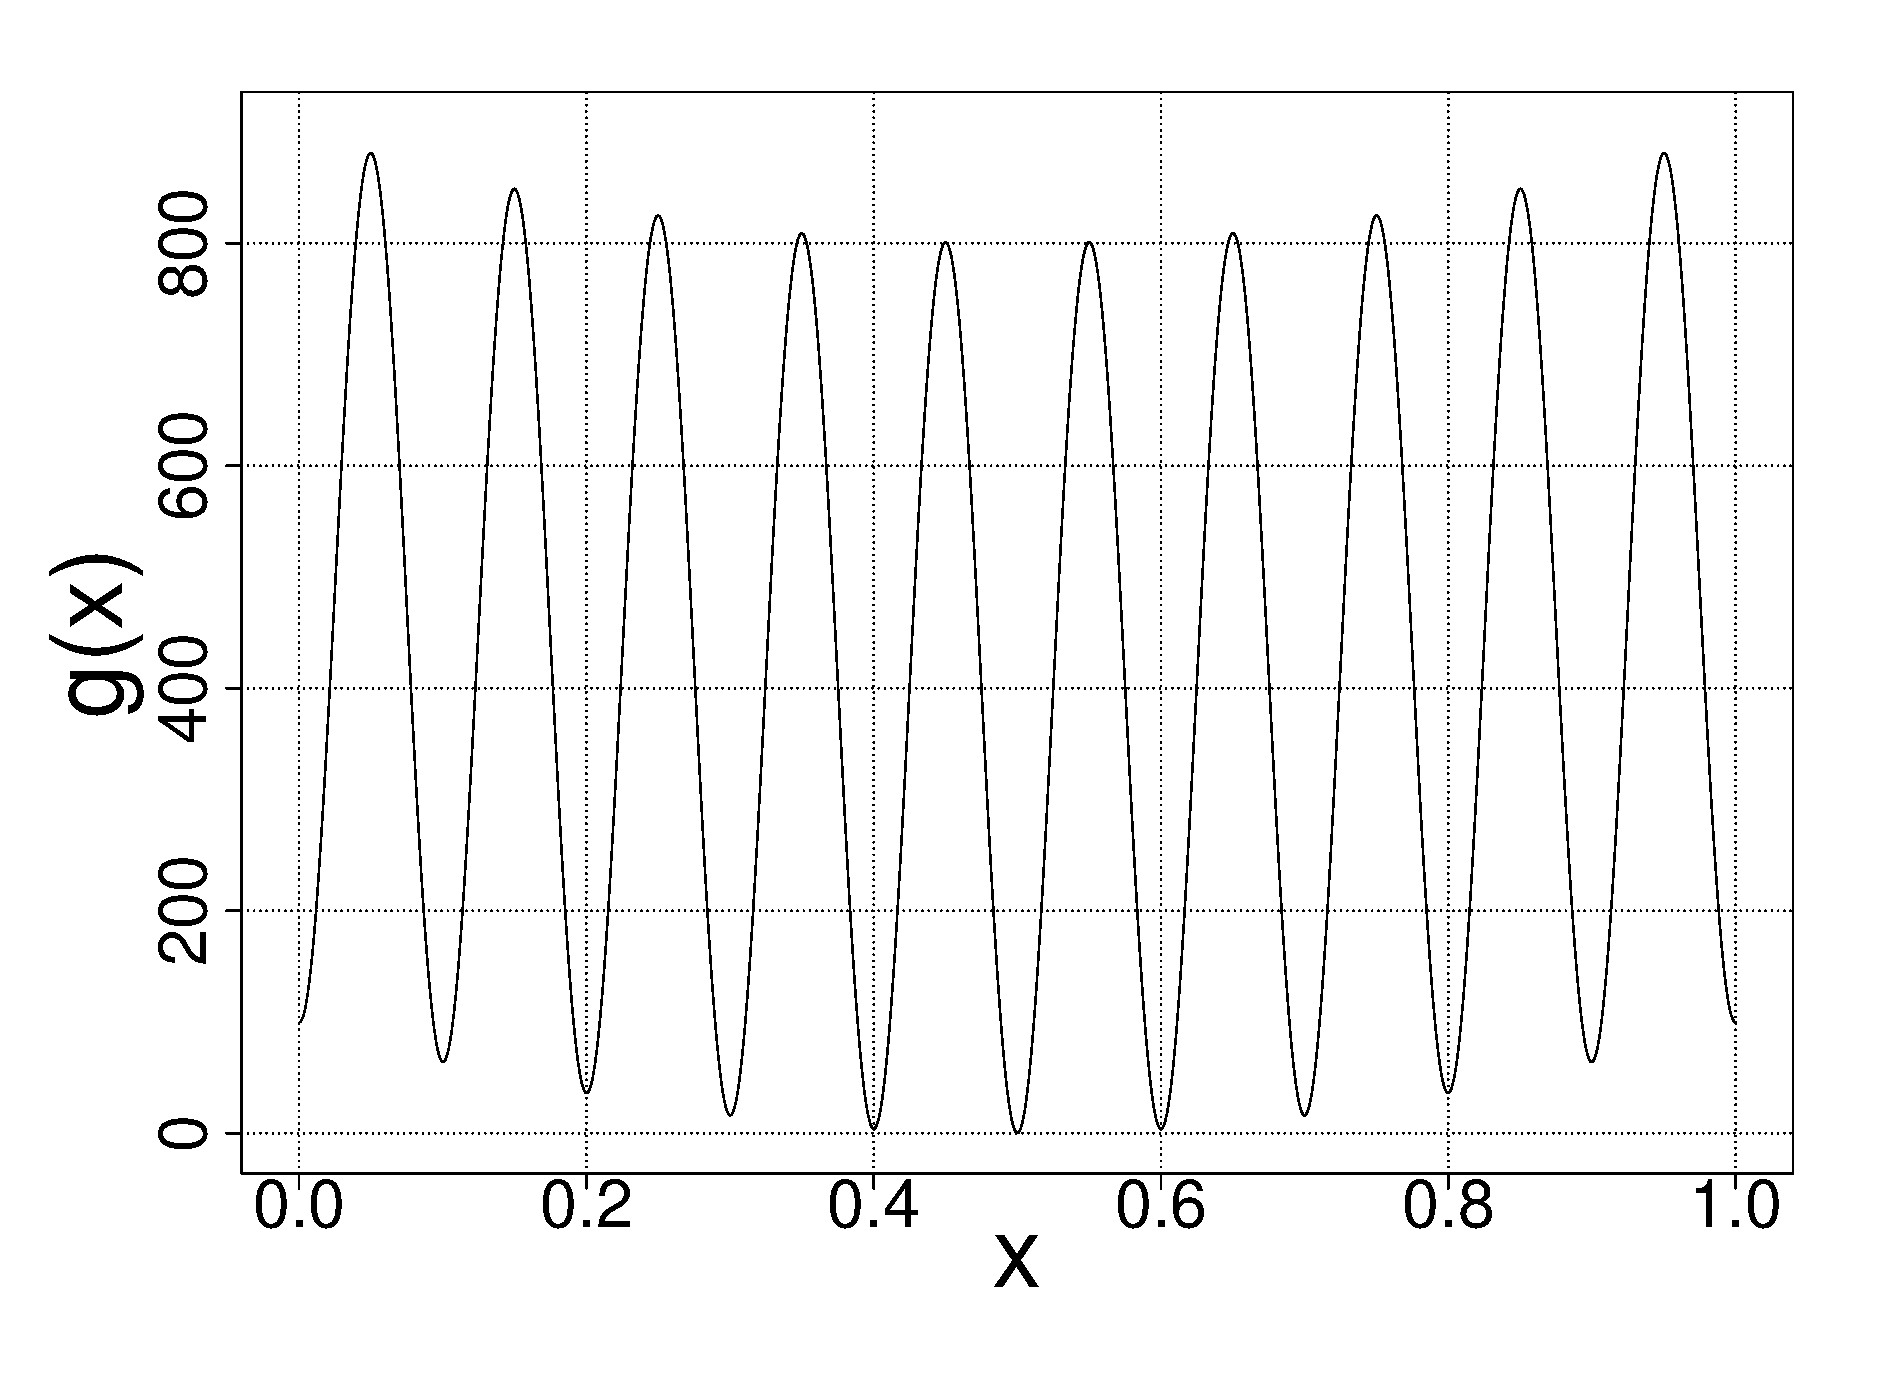
\includegraphics[width=0.65\linewidth]{../figures/DTLZ3_gx.eps}
\end{center}
\setlength{\abovecaptionskip}{-8mm}
\setlength{\belowcaptionskip}{0mm}
\caption{$g(\bm{x}_M)$の推移}
\label{fig:dtlz3_gx}
\end{figure}

\clearpage
\subsubsection{DTLZ4}
DTLZ4は  \Eqref{dtlz4}  で表される多目的問題である.
DTLZ2と基本的な構造は同様である.
DTLZ2と大きく違う点は,各目的関数$f_m$内の位置変数$x_1,\cdots,x_{M-1}$が$\alpha$乗となっている点である.
これにより,変数の値の僅かな違いが目的関数の値に大きな影響を与え,解の多様性維持のためには位置変数を高い精度で探索する必要がある.
例として$\alpha=100$の場合の$x^\alpha$と$x$の対応を\Figref{dtlz4_x} に示す.

\Figref{dtlz4_x}より,$x < 0.9$の時,$x^\alpha$はほぼ0となってしまうため,$x > 0.9$を細かく調べる必要がある.
DTLZ4のパレートフロント上の設計変数は,位置変数の$\alpha$乗$x^\alpha _1,\cdots,x^\alpha _{M-1}$が[0,1]に一様に広がっており,$g(\bm{x}_M)$が$0$,すなわちすべての距離変数$x_M,\cdots,x_n$が$0.5$となる.

\begin{eqnarray} 
\left.
\begin{array}{ll}
Min. \quad f_{1}  (\bm{x}) = (1+g(\bm{x}_{M}))\cos({x_{1}}^\alpha\pi/2)  \cdots  \cos({x_{M-2}}^\alpha\pi/2)\cos({x_{M-1}}^\alpha\pi/2),\\
Min. \quad f_{2} (\bm{x}) = (1+g(\bm{x}_{M}))\cos({x_{1}}^\alpha\pi/2)  \cdots  \cos({x_{M-2}}^\alpha\pi/2)\sin({x_{M-1}}^\alpha\pi/2), \\
Min. \quad f_{3} (\bm{x}) = (1+g(\bm{x}_{M}))\cos({x_{1}}^\alpha\pi/2)  \cdots  \sin({x_{M-2}}^\alpha\pi/2), \\
     \  \  \ $\vdots$    \qquad     \qquad      \qquad     \qquad \vdots \\
Min. \quad f_{M}(\bm{x}) = (1+g(\bm{x}_{M}))\sin({x_{1}}^\alpha\pi/2)\\
with \quad g(\bm{x}_{M}) = \sum_{x_i \in \bm{x}_M} (x_i - 0.5)^2  \\
  \qquad    \qquad    \qquad  \quad      0 \le x_{i} \le 1,  for \ i = 1, 2, \ldots, n. \\
        \qquad    \qquad    \qquad  \quad        \bm x = (x_1,x_2, \ldots, x_n)\\
   \qquad    \qquad    \qquad  \quad        \bm{x}_M = (x_M,x_{M+1}, \ldots, x_n)
   \label{dtlz4} 
\end{array}
\right\}
\end{eqnarray}


\begin{figure}[htbp]
\begin{center}
\centering
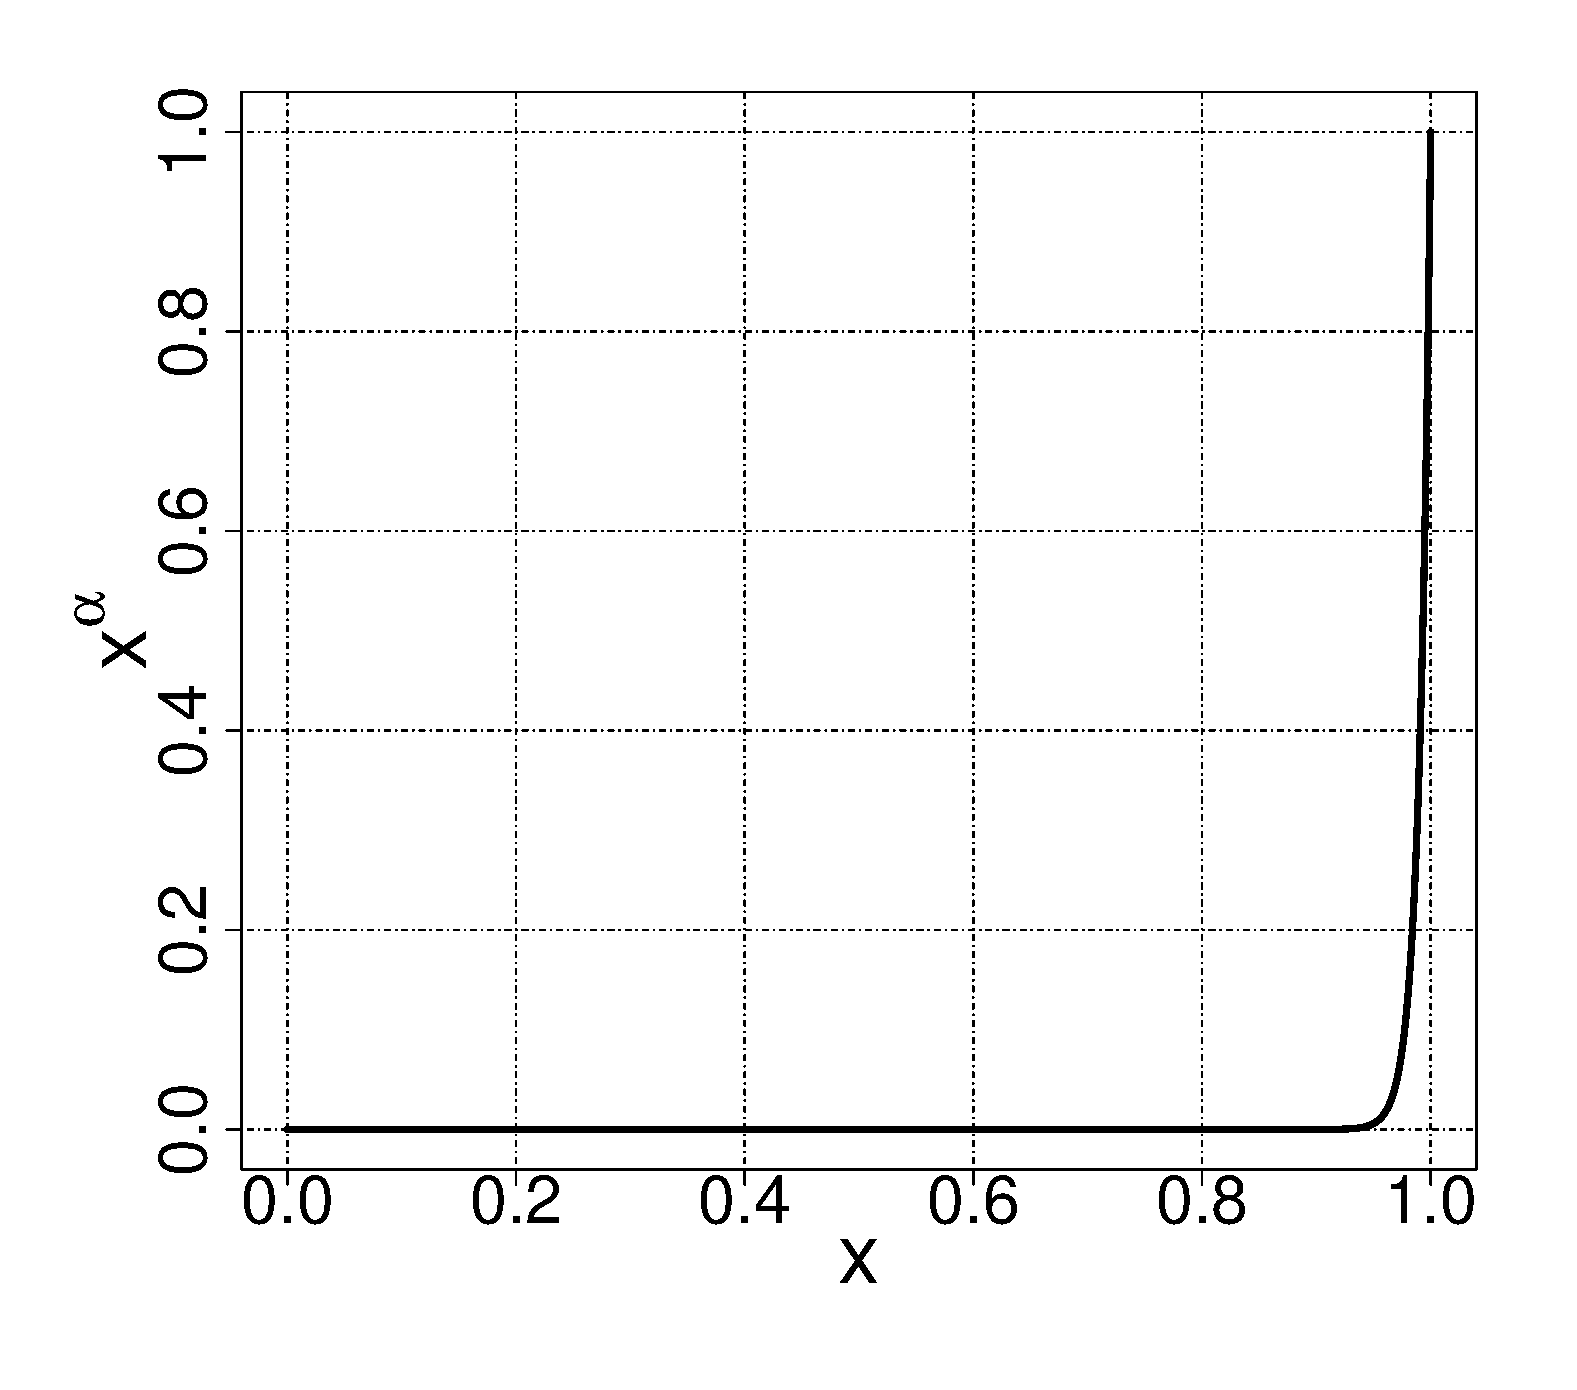
\includegraphics[width=0.4\linewidth]{../figures/dtlz4_position_sensitive.eps}
\end{center}
\setlength{\abovecaptionskip}{-8mm}
\setlength{\belowcaptionskip}{0mm}
\caption{$x$ と$x^ \alpha$の対応}
\label{dtlz4_x}
\end{figure}

\subsubsection{DTLZ7}
DTLZ7は  \Eqref{dtlz7}  で表される多目的問題である.
DTLZ7は,局所解を持たない単峰性の最適化問題であり,$M$目的の最適化問題として定式化した場合,$2^{M-1}$個の非連続な最適解部分を持つ問題である.
DTLZ2-4と同様に,設計変数$x_1,\cdots,x_{M-1}$は位置変数,設計変数$x_M,\cdots,x_n$は距離変数となるが,DTLZ2-4と異なり,距離変数$x_M$の最適値は$0$である.
したがって,DTLZ7の真のパレート最適解を得るためには,位置変数$x_1,\cdots,x_{M-1}$が一様に広がっており,すべての距離変数$x_M,\cdots,x_n$が$0$となる必要がある.

\begin{eqnarray} 
\left.
\begin{array}{ll}
Min. \quad f_{1}  (x_1) = x_1,\\
Min. \quad f_{2} (x_2) = x_2, \\
Min. \quad f_{3} (x_3) = x_3, \\
     \  \  \ $\vdots$    \qquad       \qquad \vdots \\
Min. \quad f_{M_1}(x_{M-1}) = x_{M-1},\\
Min. \quad f_{M} (\bm x) = (1 + g(\bm{x_M}))h(f_1,f_2,\cdots,f_{M-1},g),\\
with\ g(\bm{x}_{M}) = 1 + \cfrac{9}{|\bm{x_M}|} \sum_{x_i \in \bm{x_M}} x_i,  \\
\quad \quad \ h(f_1,f_2,\cdots,f_{M-1},g) = M - \sum^{M-1}_{i = 1}\left[ \cfrac{f_i}{1+g} (1 + sin(3\pi f_i))\right],\\
   \qquad    \  0 \le x_{i} \le 1,  for\ i = 1, 2, \ldots, n, \\
      \qquad    \        \bm x = (x_1,x_2, \ldots, x_n),\\
   \qquad    \        \bm{x}_M = (x_M,x_{M+1}, \ldots, x_n).
   \label{dtlz7} 
\end{array}
\right\}
\end{eqnarray}

\newpage

\subsection{WFG問題}
WFG問題\cite{}は2006年にHubandらが提案した多目的ベンチマーク問題である.
大きな特徴として,1)設計変数が何度もスケーリングされる,2)設計変数間で相関関係を持つ問題がある,3)真のパレートフロントの形状が複雑であるといった点があげられる.

上述の1点目の性質より,非常に非線形性の強い問題であり,また2点目の性質より設計変数間で相関関係を持つ場合があるため,DTLZ問題と比較し,非常に複雑な構造となっている.

基本的な式の構造は\Eqref{wfg_standard}で表される.

\begin{eqnarray} 
\left.
\begin{array}{rccl}
Min. & f_{m = 1:M}  (\bm{x}) &=& x_M + S_m h_m (x_1, \cdots, x_{M-1})\\
where & \bm{x} &=& \{x_1, \cdots, x_M\} \\
&&=& \{ max(t^p_M,A_1)(t^p_1 - 0.5) + 0.5, \cdots, \\
& & & \ \ max(t^p_M,A_{M-1})(t^p_{M-1} - 0.5)+0.5, t^p_M\} \\
& \bm{t^p} &=& \{t^p_1, \cdots, t^p_M \} \longleftarrow [ \ \bm{t^{p-1}} \longleftarrow [ \ \cdots \longleftarrow [ \ \bm{t^1} \longleftarrow [ \ \bm{z_{[0,1]}}\\
&  \bm{z_{[0,1]}} &=& \{ z_{1,[0,1]}, \cdots, z_{n,[0,1]} \} = \{ z_1 / z_{1,max}, \cdots, z_n / z_{n,max} \}
   \label{wfg_standard} 
\end{array}
\right\}
\end{eqnarray}

\Eqref{wfg_standard}において,$M$は目的関数の数を示している.
$\bm{x}$は目的関数値を定める値で$M$個からなり,$x_1, \cdots, x_{M-1}$が目的関数空間における解の位置を決定する値,$x_M$が目的関数空間における解の原点からの距離を決定する値となる.
$\bm{z}$は,設計変数値を表し,設計変数の数$n$は位置パラメータ$k$と距離パラメータ$l$を足した数となる.
$A_{1:M-1}$は0または1の定数であり問題によって決定される.
$h_{1:M}$はパレートフロントの形状を決定する関数(形状関数),$S_{1:M}$はスケーリングを行う定数である.
$t^{1:p}$は,射影変換された変数を示し,$\longleftarrow$は後述するスケーリング関数を用いて変数を射影することを意味する.

このように,WFG問題では,設計変数$\bm{z}$を何度もスケーリング(射影)し,$t^p$に変換したのち,目的関数値を定める$\bm{x}$を算出し,パレートフロントの形状を決定する関数$h_{1:M}$に与えることで,目的関数値が算出される.

本研究で用いるWFG2,4,6,7で使用される形状関数$h_{1:M}$とスケーリング関数をそれぞれ\Tabref{wfg_shape},\Tabref{wfg_trans}にそれぞれまとめる.

また,WFG2,4,6,7で使用する形状関数$h_{1:M}$とスケーリング関数の組み合わせを\Tabref{wfg_comb}に示す.



\begin{table}[htbp]
\fontsize{9.5pt}{9.5pt} \selectfont
%\tabcolsep = 1pt
\centering
\caption{本研究で用いるWFG問題で使用される形状関数}
\vspace{0.1cm}
\label{wfg_shape}
\begin{tabular}{|c|}
\hline 
$\bf{Convex}$\\
\hline
$convex_1(x_1, \cdots, x_{M-1}) = \prod^{M-1}_{i=1} (1 - cos(x_i \pi / 2 )) $\\
$convex_{m=2:M-1}(x_1, \cdots, x_{M-1}) =\left( \prod^{M-m}_{i=1} (1 - cos(x_i \pi / 2 )) \right) ( 1 - sin(x_{M-m-1} \pi / 2 ) )$\\
$convex_M(x_1, \cdots, x_{M-1}) = 1 - sin( x_1 \pi / 2 )$\\
%When $h_{m = 1:M} = convex_m$, the Pareto optimal front is purely convex.\\
\hline
\hline
$\bf{Concave}$\\
\hline
$concave_1(x_1, \cdots, x_{M-1}) = \prod^{M-1}_{i=1} (1 - cos(x_i \pi / 2 )) $\\
$concave_{m=2:M-1}(x_1, \cdots, x_{M-1}) =\left( \prod^{M-m}_{i=1} (1 - cos(x_i \pi / 2 )) \right) ( 1 - sin(x_{M-m-1} \pi / 2 ) )$\\
$concave_M(x_1, \cdots, x_{M-1}) = 1 - sin( x_1 \pi / 2 )$\\
%When $h_{m = 1:M} = concave_m$, the Pareto optimal front is purely concave, and a region of the hyper-sphere\\
%of radius one centered at the origin, where $\Sigma^M_{m=1} h^2_m = 1$.\\
\hline
\hline
${\bf Disconnected} (\alpha, \beta > 0, A \in \{1, 2, \cdots \}) $\\
\hline
$disc_M (x_1, \cdots, x_{M-1}) = 1 - (x_1)^\alpha cos^2 (A(x_1)^\beta \pi)$\\
\hline
\end{tabular}
\end{table}


\begin{table}[htbp]
\fontsize{9.5pt}{9.5pt} \selectfont
%\tabcolsep = 1pt
\centering
\caption{本研究で用いるWFG問題で使用されるスケーリング関数}
\vspace{0.1cm}
\label{wfg_trans}
\begin{tabular}{|c|}
\hline 
${\bf Bias : Parameter Dependent} (A \in (0,1), 0 < B < C)$\\
\hline
$b\_param(y, \bm{y}\prime, A, B, C) = y^{B+(C-B) v ( u (\bm{y} \prime ))}$\\
$v ( u (\bm{y} \prime )) = A - (1 - 2 u (\bm{y} \prime )) \left| \lfloor 0.5 - u (\bm{y} \prime ) \rfloor + A \right|$\\
\hline
\hline
${\bf Shift : Linear} (A \in (0,1))$\\
\hline
$s\_linear(y, A) = \cfrac{|y - A|}{|\lfloor A - y \rfloor + A|}$\\
\hline
\hline
{\bf Shift : Multi-modal} $(A \in \{1, 2, \cdots\}, B \geq 0, (4A + 2)\pi \geq 4B, C \in (0,1)) $\\
\hline
$s\_multi(y, A, B, C) = \cfrac{1 + cos \left[ (4A+2) \pi \left( 0.5 - \cfrac{|y - C|}{2(\lfloor C - y \rfloor + C)} \right) \right] + 4B \left( \cfrac{|y - C|}{2(\lfloor C - y \rfloor + C) }  \right) ^ 2}{B+2}$\\
\hline
\hline
{ \bf Reduction : Weighted Sum} $(|\bm{w}| = |\bm{y}|, w_1, \cdots, w_{|\bm{y}|}) $\\
\hline
$r\_sum (\bm{y}, \bm{w}) =  \left( \Sigma^{|\bm{y}|}_{i=1} w_i y_i \right) / \Sigma^{|\bm{y}|}_{i=1} w_i$\\
\hline
\hline
{\bf Reduction : Non-separable} $(A \in \{1,  \cdots, |\bm{y}| \}, |\bm{y}| \ mod \ A = 0) $\\
\hline
$r\_nonsep (\bm{y}, A) = \cfrac{\Sigma^{|\bm{y}|}_{j=1}\left(  y_j + \Sigma^{A-2}_{k=0} \left| y_j - y_{1 + (j + k) \ mod \  | \bm{y} | } \right| \right)}{\cfrac{|\bm{y}|}{A} \lceil A / 2 \rceil (1 + 2A - 2 \lceil A / 2 \rceil)}$\\
\hline
\end{tabular}
\end{table}

\begin{table}[htbp]
\fontsize{10pt}{10pt} \selectfont
%\tabcolsep = 1pt
\centering
\caption{本研究で用いるWFG問題の形状関数とスケーリング関数の組み合わせ}
\label{wfg_comb}
\begin{tabular}{|c||c|l|}
\hline
Problem & Type & \multicolumn{1}{c|}{Setting}\\
\hline
All & Constants & $S_{m=1:M} = 2m$\\
&                       & $A_{1:M-1} = 1$ ( for WFG 2, 4, 6 and 7)\\
\hline
All & Domains & $z_{i = 1:n,max} = 2i$\\
\hline
WFG2 & Shape & $h_{m = 1:M-1} = convex_m$\\
           &             & $h_M = disc_M ( with \alpha = \beta = 1 \ and \ A = 5)$\\
           &     $t^1$   & $t^1_{i=1:k} = y_i$\\
           &             &$ t^1_{i = k+1:n} = s\_linear(y_i, 0.35)$\\
           &     $t^2$    & $t^2_{i = 1:k} = y_i$\\
           &             & $t^2_{i = k+1:k+l/2} = r\_nonsep(\{ y_{k+2(i - k) - 1}, y_{k+2(i - k)} \},2)$\\
           &     $t^3$    & $t^3_{i = 1:M-1} = r\_sum(\{ y_{(i-1)k / (M - 1) + 1}, \cdots, y_{ik / (M-1)} \}, \{1, \cdots, 1 \} )$\\
           &              & $t^3_M = r\_sum(\{ y_{k+1}, \cdots, y_{k+l/2} \} , \{ 1, \cdots, 1\} )$\\
\hline
WFG4 & Shape &$ h_{m = 1:M} = concave_m$\\
           &     $ t^1$  & $t^1_{i = 1:n} = s\_multi(y_i , 30, 10, 0.35)$\\
           &  $t^2$      & $t^2_{i = 1:M-1} = r\_sum(\{ y_{(i-1)k / (M - 1) + 1}, \cdots, y_{ik / (M-1)} \}, \{1, \cdots, 1 \} )$\\
           &                 & $t^2_M = r\_sum(\{ y_{k+1}, \cdots, y_n  \}, {1, \cdots, 1})$\\
\hline
WFG6 & Shape & $h_{m = 1:M} = concave_m$\\
           &     $t^1$   & As $t^1$ from WFG2. (Linear shift.)\\
           &     $t^2$    & $t^2_{i = 1:M-1} = r\_nonsep(\{ y_{(i - 1)k/(M-1)+1},\cdots, y_{ik/(M-1)} \}, k/(M-1))$\\
           &             & $t^2_M = r\_nonsep(\{ y_{k+1},\cdots, y_{n} \},l)$\\
\hline
WFG7 & Shape & $h_{m = 1:M} = concave_m$\\
           &     $ t^1$  & $t^1_{i = 1:k} = b\_param(y_i , r\_sum(\{ y_{i+1}, \cdots, y_n \}, \{1, \cdots, 1\}), \cfrac{0.98}{49.98},0.02,50)$\\
           &                 & $ t^1_{i = k+1:n} = y_i$\\
           &     $t^2$   & As $t^1$ from WFG2. (Linear shift.)\\
           &     $t^3$   & As $t^2$ from WFG4. (Weighted sum reduction.)\\
\hline  
WFG8 & Shape & $h_{m = 1:M} = concave_m$\\
           &     $ t^1$  & $t^1_{i = 1:k} = y_i$\\
           &                 & $t^1_{i = k+1:n} = b\_param(y_i , r\_sum(\{ y_{i+1}, \cdots, y_n \}, \{1, \cdots, 1\}), \cfrac{0.98}{49.98},0.02,50)$\\
           &     $t^2$   & As $t^1$ from WFG2. (Linear shift.)\\
           &     $t^3$   & As $t^2$ from WFG4. (Weighted sum reduction.)\\
\hline  
\end{tabular}
\end{table}

\clearpage

\subsection{CEC2009問題}
CEC2009問題\cite{}は2009年にZhangらが提案した多目的ベンチマーク問題である.
CEC2009問題は現実の設計問題に近い問題を作成するという意図で提案された.
現実の設計問題に近い構成にするため,設計変数同士に相関を持つことや,制約条件が存在する,真のパレートフロントが不連続な形状をしている等複雑な構成となっていることが特徴である.
CEC2009問題は20種類のベンチマーク問題があり,その内10種類は制約条件付き問題である.
本研究では,制約なしのベンチマーク問題であるUF2,UF9と制約条件付きベンチマーク問題であるCF2,CF7の4つのベンチマーク問題で数値実験を行う.
次節以降でこれら4つのベンチマーク問題について述べる.

\subsubsection{UF2}
UF2は制約なしの2目的のベンチマーク問題である.
\Eqref{uf2_eq}にUF2の構成を示す.
設計変数の数$n$は任意に決定することができ,設計変数の探索領域は$[0,1] \times [-1,1]^{n-1}$となる.
%また,真のパレートフロントの形状を\Figref{}に示す.

\begin{eqnarray} 
\left.
\begin{array}{rccl}
Min. &f_1 &=& x_1 + \cfrac{2}{|\bm{J_1}|} \sum_{j \in \bm{J_1}} y^2_j\\
Min. & f_2 &=& 1 - \sqrt{x_1} + \cfrac{2}{|\bm{J_2}|} \sum_{j \in \bm{J_2}} y^2_j\\

where &  \bm{J_1} &=& \{j|j {\rm \ is \ odd \ and \ } 2 \leq j \leq n\}\\
& \bm{J_2} &=& \{j|j {\rm \ is \ even \ and \ } 2 \leq j \leq n\}\\
& y_j &=& \left\{ 
\begin{array}{l}
x_j - [0.3 x^2_1 cos (24 \pi x_1 + \frac{4j\pi}{n}) + 0.6x_1] \\
\qquad \qquad \qquad \qquad \times cos(6 \pi x_1 + \frac{j \pi}{n}) \ \ j \in \bm{J_1}\\
x_j - [0.3 x^2_1 cos (24 \pi x_1 + \frac{4j\pi}{n}) + 0.6x_1]\\
\qquad \qquad \qquad \qquad \times sin(6 \pi x_1 + \frac{j \pi}{n}) \ \ j \in \bm{J_2}\\
\end{array}
\right.
   \label{uf2_eq} 
\end{array}
\right\}
\end{eqnarray}


\subsubsection{UF9}
UF9は制約なしの3目的のベンチマーク問題である.
\Eqref{uf9_eq}にUF9の構成を示す.
設計変数の数$n$は任意に決定することができ,設計変数の探索領域は$[0,1]^2 \times [-2,2]^{n-2}$となる.

\begin{eqnarray} 
\left.
\begin{array}{rccl}
Min. & f_1 &=& 0.5[max\{0, (1 + \epsilon)(1 - 4(2x_1 - 1)^2)\} + 2x_1]x_2 \\
                     &&&                             + \cfrac{2}{|\bm{J_1}|} \sum_{j \in \bm{J_1}}(x_j - 2x_2 sin(2 \pi x_1 + \cfrac{j \pi}{n} ))^2\\
Min. & f_2 &=& 0.5[max\{0, (1 + \epsilon)(1 - 4(2x_1 - 1)^2)\} - 2x_1 + 2]x_2 \\
                      &&&                             + \cfrac{2}{|\bm{J_2}|} \sum_{j \in \bm{J_2}}(x_j - 2x_2 sin(2 \pi x_1 + \cfrac{j \pi}{n} ))^2\\
Min. & f_3 &=& 1-x_2 \\
                                            &&&+ \cfrac{2}{|\bm{J_3}|} \sum_{j \in \bm{J_3}}(x_j - 2x_2 sin(2 \pi x_1 + \cfrac{j \pi}{n} ))^2\\

where &  \bm{J_1} &=& \{j|3 \leq j \leq n, {\rm \ and \ } j - 1 {\rm \ is \ a \ multiplication \ of \ \ } 3\}\\
& \bm{J_2} &=& \{j|3 \leq j \leq n, {\rm \ and \ } j - 2 {\rm \ is \ a \ multiplication \ of \ \ } 3\}\\
& \bm{J_3} &=& \{j|3 \leq j \leq n, {\rm \ and \ } j {\rm \ is \ a \ multiplication \ of \ \ } 3\}\\
&  \epsilon &=& 0.1

   \label{uf9_eq} 
\end{array}
\right\}
\end{eqnarray}

\subsubsection{CF2}
CF2は1制約2目的のベンチマーク問題である.
\Eqref{cf2_eq}にCF2の構成を示す.
設計変数の数$n$は任意に決定することができ,設計変数の探索領域は$[0,1] \times [-1,1]^{n-1}$となる.

\begin{eqnarray} 
\left.
\begin{array}{rccl}
Min. & f_1 &=& x_1 + \cfrac{2}{|\bm{J_1}|} \sum_{j \in \bm{J_1}}(x_j - sin(6\pi x_1 + \cfrac{j\pi}{n}))^2\\
Min. &f_2 &=& 1 - \sqrt{x_1} + \cfrac{2}{|\bm{J_2}|} \sum_{j \in \bm{J_2}} (x_j - cos(6\pi x_1 + \cfrac{j\pi}{n}))^2\\

where &  \bm{J_1} &=& \{j|j {\rm \ is \ odd \ and \ } 2 \leq j \leq n\}\\
& \bm{J_2} &=& \{j|j {\rm \ is \ even \ and \ } 2 \leq j \leq n\}\\
const. & c_1(\bm x) & = &\cfrac{t}{1 + e^{4|t|}} \geq 0\\
where & t &=& f_2 + \sqrt{f_1} - a sin[N\pi (\sqrt{f_1} - f_2 + 1)] - 1\\
   \label{cf2_eq} 
\end{array}
\right\}
\end{eqnarray}


\subsubsection{CF7}
CF7は2制約2目的のベンチマーク問題である.
\Eqref{cf7_eq}にCF7の構成を示す.
設計変数の数$n$は任意に決定することができ,設計変数の探索領域は$[0,1] \times [-2,2]^{n-1}$となる.

\begin{eqnarray} 
\left.
\begin{array}{rccl}
Min. & f_1 &=& x_1 + \sum_{j \in \bm{J_1}} h_j(y_j)\\
Min. & f_2 &=& (1 - x_1)^2 + \sum_{j \in \bm{J_2}} h_j(y_j)\\
where &  \bm{J_1} &=& \{j|j {\rm \ is \ odd \ and \ } 2 \leq j \leq n\}\\
           & \bm{J_2} &=& \{j|j {\rm \ is \ even \ and \ } 2 \leq j \leq n\}\\
           & y_j &=& \left\{ 
\begin{array}{l}
x_j - cos (6 \pi x_1 + \frac{j\pi}{n}) \ \ j \in \bm{J_1}\\
x_j - sin (6 \pi x_1 + \frac{j\pi}{n}) \ \ j \in \bm{J_2}\\
\end{array}
\right. \\
&h_2(t) &=& h_4(t) = t^2\\
&h_j(t) &=& 2t^2 - cos(4\pi t) + 1 \ \ \ {\rm for \ } \ j = 3,5,6, \cdots, n \\
const. & c_1(\bm x) &=& x_2 - sin(6 \pi x_1 + \cfrac{2\pi}{n}) \\
                        &&&      - Sgn(0.5(1-x_1) - (1-x_1)^2)\\
                        &&& \times \sqrt{|0.5(1-x_1) - (1-x_1)^2|} \geq 0\\
&    c_2(\bm x) & = &x_4 - sin(6\pi x_1 + \cfrac{4\pi}{n}) \\
                    &&& - Sgn(0.25\sqrt{1-x_1} - 0.5(1-x_1))\\
                    &&& \times \sqrt{|0.25 \sqrt{1-x_1} - 0.5(1-x_1)|} \geq 0\\
   \label{cf7_eq} 
\end{array}
\right\}
\end{eqnarray}

\newpage

\subsection{CDTLZ問題}
CDTLZ問題\cite{}は2014年にJainらによって提案された制約条件付きのベンチマーク問題である.
CDTLZ問題はDebらが考案したDTLZ問題に制約条件を追加した問題であり,6つの問題が提案されている.
CDTLZ問題では,3種類の制約条件の問題が用意されている.

C1シリーズの問題は,オリジナルのDTLZ問題の真のパレートフロントを覆うように実行不可能領域が存在する問題であり,実行不可能領域を越えなければ真のパレートフロントに到達できないため,実行不可能領域と実行可能領域の境界付近に局所最適解が生成されやすい.
C2シリーズの問題は,オリジナルのDTLZ問題の真のパレートフロント上に部分的に実行不可能領域が存在する問題であり,真のパレートフロントの形状が不連続となる.
C3シリーズの問題は,オリジナルのDTLZ問題の真のパレートフロントが実行不可能領域に存在する問題であり,実行可能領域と実行不可能領域の境界線が真のパレートフロントとなる.

本研究では,C1DTLZ3,C2DTLZ2 convex,C3DTLZ1の3つの問題を数値実験に使用した.
次節以降でこれらの問題について説明する.

\subsubsection{C1DTLZ3}
C1DTLZ3はDTLZ3に1つ制約条件を追加したベンチマーク問題である.
真のパレートフロントを覆うように実行不可能領域が存在し,実行可能領域と実行不可能領域の境界付近に局所最適解が生成されやすい問題となっている.
C1DTLZ3で追加された制約条件を\Eqref{c1dtlz3_const}に示す.
本実験では$r$を$9$とした.

\begin{equation}
\centering
c(\bm{x}) = \left( \sum^M_{i=1} f_i (\bm{x})^2 - 16 \right) \left( \sum^M_{i=1} f_i(x)^2 - r^2 \right) \geq 0
\label{c1dtlz3_const}
\end{equation}


\subsubsection{C2DTLZ2 convex}
C2DTLZ2 convexはDTLZ2のパレートフロントの形状を凹型から凸型に変更し,1つ制約条件をを追加したベンチマーク問題である.
真のパレートフロント上に部分的に実行不可能領域が存在し,実行可能な真のパレートフロントの形状は不連続となっている.
C2DTLZ convexで変更された目的関数の射影変換を\Eqref{c2dtlz2_changed}に,追加された制約条件を\Eqref{c2dtlz2_const}に示す.
本実験では$r$を$0.225$とした.

\begin{eqnarray}
\left.
\begin{array}{rcl}
f_i &\longleftarrow& f^4_i \ \ \ \ i = 1, 2, \cdots, M-1\\
f_M &\longleftarrow& f^2_M
\end{array}
\right\}
\label{c2dtlz2_changed}
\end{eqnarray}

\begin{eqnarray}
\left.
\begin{array}{rcl}
c(\bm{x}) &=& \sum^M_{i=1} (f_i(\bm{x}) - \lambda)^2 - r^2 \geq 0\\
where \ \ \lambda &=& \cfrac{1}{M} \sum^M_{i=1} f_i(\bm{x})\\
\end{array}
\right\}
\label{c2dtlz2_const}
\end{eqnarray}

\subsubsection{C3DTLZ1}
C3DTLZ1はDTLZ1に目的関数の数$M$だけ制約条件を追加したベンチマーク問題である.
DTLZ1の真のパレートフロントが実行不可能領域にあり,実行可能領域と実行不可能領域の境界線がパレート最適解となる問題である.
C3DTLZ1で追加された制約条件を\Eqref{c3dtlz1_const}に示す.

\begin{equation}
c_j(\bm{x}) = \sum^M_{i = 1, i \neq j} f_j(\bm{x}) + \cfrac{f_i(\bm x)}{0.5} - 1 \geq 0 \ \ \ \ \ \forall j = 1, 2, \cdots, M
\end{equation}

\newpage

\subsection{Engineering問題}
本実験では現実の設計問題に則したEngineering問題としてCar Side Impact問題\cite{}とWelded Beam Design問題\cite{}を用いて数値実験を行った.
次節以降でこれらの問題について述べる.

\subsubsection{Car Side Impact}
Car Side Impact問題\cite{}は,3目的の最小化最適化問題である.
各目的関数にはトレードオフの関係があり,10個の制約条件と7つの設計変数を持つ問題である.
Car Side Impact問題は\Eqref{car_eq}で表される.

\subsubsection{Welded Beam Design}
Welded Beam Design\cite{}問題は,2目的の最小化最適化問題である.
各目的関数にはトレードオフの関係があり,4個の制約条件と4つの設計変数を持つ問題である.
Welded Beam Design問題は\Eqref{wbd_eq}で表される.

\begin{eqnarray}
\left.
\begin{array}{rccl}
Min. & f_1(\bm x) &=& 1.98 + 4.9 x_1 + 6.67x_2 + 6.98x_3 + 4.01x_4 + 1.78x_5 \\ 
        &                   &  & + 0.00001x_6 + 2.73x_7\\
Min. & f_2(\bm x) &=& F\\
Min. & f_3(\bm x) &=& 0.5(V_{MBP} + V_{FD})\\
const. &c_1(\bm x) &=& 1.16 - 0.3717x_2x_4 - 0.0092928x_3 \leq 1\\
          & c_2(\bm x) &=& 0.261 - 0.0159x_1x_2 - 0.006486x_1 - 0.019x_2x_7 \\
          &                    &  &+ 0.0144x_3x_5 + 0.0154464x_6 \leq 0.32\\
          & c_3(\bm x) &=& 0.214 + 0.00817x_5 - 0.045195x_1 - 0.0135168x_1 \\
          &                    &   &+ 0.03099x_2x_6 - 0.018x_2x_7 + 0.007176x_3 + 0.023232x_3 \\
          &                    &   &- 0.00364x_5x_6 - 0.018x_2^2 \leq 0.32\\
          & c_4(\bm x) &=& 0.74 - 0.61x_2 - 0.031296x_3 - 0.031872x_7 \\
          &                    &  &+ 0.227x_2^2 \leq 0.32\\
          & c_5(\bm x) &=& 28.98 + 3.818x_3 - 4.2x_1x_2 + 1.27296x_6 \\
          &                   &   &- 2.68065x_7 \leq 32\\
          & c_6(\bm x) &=& 33.86 + 2.95x_3 - 5.057x_1x_2 - 3.795x_2 \\
          &                   &   &- 3.4431x_7 + 1.45728 \leq32\\
          & c_7(\bm x) &=& 44.36 - 9.9x_2 - 4.4505x_1 \leq 32\\
          & c_8(\bm x) &\equiv & F = 4.72 - 0.5x_4 - 0.19x_2x_3 \leq4\\
          & c_9(\bm x) & \equiv & V_{MBP} = 10.58 - 0.674x_1x_2 - 0.067275x_2 \leq 9.9\\
          & c_{10}(\bm x) & \equiv & V_{FD} = 16.45 - 0.489x_3x_7 - 0.843x_5x_6 \leq 15.7\\
where & & & 0.5 \leq x_1 \leq 1.5, 0.45 \leq x_2 \leq 1.35, 0.5 \leq x_3 \leq 1.5\\
           & & & 0.5 \leq x_1 \leq 1.5, 0.875 \leq x_5 \leq 2.625, 0.4 \leq x_6 \leq 1.2,\\
           & & & 0.4 \leq x_7 \leq 1.2\\
\end{array}
\right\}
\label{car_eq}
\end{eqnarray}

\begin{eqnarray}
\left.
\begin{array}{rccl}
Min. & f_1(\bm x) &=& 1.10471h^2l + 0.04811tb(14.0 + l) \\ 
Min. & f_2(\bm x) &=& \cfrac{2.1952}{t^3b}\\
const. &c_1(\bm x) &\equiv& 13,600 - \tau(\bm x) \geq 0\\
          & c_2(\bm x) &\equiv& 30,000 - \sigma(\bm x) \geq 0 \\
          & c_3(\bm x) &\equiv& b-h \geq 0 \\
          & c_4(\bm x) &\equiv& P_c(\bm x) - 6,000 \geq 0\\

where &\tau(\bm x) & = & \sqrt{(\tau^\prime) + (\tau^{\prime \prime})^2 + (l \tau^\prime \tau^{\prime \prime}) / \sqrt{0.25(l^2 + (h+t)^2)}}\\
           &\tau^\prime & = & \cfrac{6,000}{\sqrt{2}hl}\\
           &\tau^{\prime \prime} &=& \cfrac{6,000(14 + 0.5l)\sqrt{0.25(l^2 + (h+t)^2)}}{2\{0.707hl(l^2/12+0.25(h+t)^2)\}}\\
           &\sigma(\bm x) &=& \cfrac{504,000}{t^2b}\\
           &P_c(\bm x) &=& 64,746.022(1-0.0282346t)tb^3\\
           & \bm x &=& (h, b, l, t)\\
           & & & 0.125 \leq h,b \leq 5.0, 0.1 \leq l,t \leq 10.0\\
\end{array}
\right\}
\label{wbd_eq}
\end{eqnarray}

\newpage

\subsection{Modified DTLZ問題}
Modified DTLZ問題\cite{}は2017年に近藤らによって提案されたベンチマーク問題である.
Modified DTLZ問題はDebらが考案したDTLZ問題を改変したものであり,3つの問題が提案されている.
オリジナルのDTLZ問題では上述の通り距離変数が0.5となった時に真のパレートフロントに到達する.
しかし,これでは設計変数の小数点以下の桁数を小さくするほど,真の最適値に用意に収束してしまうと考えられる.
Modified DTLZ問題では,距離変数の最適値を無理数に変更することで,小数点以下の桁数を粗くしただけでは収束しづらい問題となっている.
次節よりModified DTLZ2-4について述べる.

\subsubsection{Modified DTLZ2, 4}
Modified DTLZ2,4は,DTLZ2,4の距離変数の最適値を$0.5$から無理数である$0.1\pi$に変更したものである.
DTLZ2,4では$g(\bm x)$は\Eqref{gx_dtlz2}で定義される.

\begin{equation}
\centering
g(\bm x_M) = \sum_{x_i \in \bm x_M} (x_i - 0.5)^2
\label{gx_dtlz2}
\end{equation}

$M$は目的関数の数を,$\bm x$は設計変数を示している.
$\bm x_M$は,設計変数の中でも距離変数と呼ばれる変数を表し,目的関数空間での真のパレートフロントまでの距離を決定する.
DTLZ2とDTLZ4では,距離変数$\bm x_M$がすべて$0.5$に収束したとき,真のパレートフロントに到達する.
上述の通り,これでは設計変数の小数点以下の桁数を小さくするほど,真の最適値に用意に収束してしまうと考えられる.
そこで,小数点以下の桁数を粗くしただけでは収束しづらいよう$g(\bm x_M)$を\Eqref{gx_mod2}とし,距離変数$\bm x_M$がすべて$0.1\pi$という無理数に収束しなければ,パレートフロントに到達しないように改変されている.

\begin{equation}
\centering
g(\bm x_M) = \sum_{x_i \in \bm x_M} (x_i - 0.1 \pi)^2
\label{gx_mod2}
\end{equation}

\subsubsection{Modified DTLZ3}
Modified DTLZ3はDTLZ3の距離変数の最適値を$0.5$から無理数である$0.1 \pi$に変更したものである.
Modified DTLZ2,4と同様に,\Eqref{gx_dtlz3}で定義される$g(\bm x_M)$より,距離変数の最適値が$0.5$となっている.
これを\Eqref{gx_mod3}に改変することで,距離変数の最適値を無理数に変更する.

\begin{equation}
\centering
g(\bm x_M) = 100[|\bm x_M| + \sum_{x_i \in \bm x_M} (x_i - 0.5)^2 - cos(20 \pi (x_i - 0.5 ))]
\label{gx_dtlz3}
\end{equation}

\begin{equation}
\centering
g(\bm x_M) = 100[|\bm x_M| + \sum_{x_i \in \bm x_M} (x_i - 0.1\pi)^2 - cos(20 \pi (x_i - 0.1 \pi ))]
\label{gx_mod3}
\end{equation}

\newpage


\subsection{Multi DTLZ問題}
Multi DTLZ問題は近藤らの提案したModified DTLZ問題をさらに改変したものである.
Modified DTLZ問題は距離変数の最適値が$0.1\pi$の1つだけである.
現実の設計問題を考えた場合,最適値が2つ以上存在する場合などが考えられるが,このような問題のベンチマーク問題は少ない.
そこで,Modified DTLZ問題を改変することで,最適値が2つとなる問題を提案する.
次節から,Multi DTLZ2,3,4について述べる.

\subsubsection{Multi DTLZ2,4}
Multi DTLZ2,4はそれぞれModified DTLZ2,4を改変したものである.
上述の\Eqref{gx_mod2}より,Modified DTLZ2,4は距離変数の最適値が$0.1\pi$の1点である.
Multi DTLZ2,4では\Eqref{gx_mod2}を\Eqref{gx_multi2}に改変することで距離変数の最適値が$0.1\pi$と$0.3\pi$の2点となる.

\begin{eqnarray}
g(\bm x_M) = 
\left\{
\begin{array}{rl}
\sum_{x_i \in \bm x_M} (x_i - 0.1 \pi)^2 & if  \ \ \  0 \leq x_i < 0.5\\
\sum_{x_i \in \bm x_M} (x_i - 0.3 \pi)^2 & otherwise \\
\end{array}
\right.
\label{gx_multi2}
\end{eqnarray}


\subsubsection{Multi DTLZ3}
Multi DTLZ3はModified DTLZ3を改変したものである.
上述の\Eqref{gx_mod3}より,Modified DTLZ3は距離変数の最適値が$0.1\pi$の1点である.
Multi DTLZ3では\Eqref{gx_mod3}を\Eqref{gx_multi3}に改変することで距離変数の最適値が$0.1\pi$と$0.3\pi$の2点となる.

\begin{eqnarray}
g(\bm x_M) = 
\left\{
\begin{array}{ll}
100[|\bm x_M| + \sum_{x_i \in \bm x_M} (x_i - 0.1\pi)^2 &\\
\qquad \qquad \qquad \qquad - cos(20 \pi (x_i - 0.1 \pi ))] & if  \  0 \leq x_i < 0.5 \\
100[|\bm x_M| + \sum_{x_i \in \bm x_M} (x_i - 0.3\pi)^2 &\\
\qquad \qquad \qquad \qquad - cos(20 \pi (x_i - 0.3 \pi ))] & otherwise \\
\end{array}
\right.
\label{gx_multi3}
\end{eqnarray}

\newpage
\section{計算条件}
\quad 本研究で用いるNSGA-IIの計算条件を \Tabref{tbl:condition} に示す.
また,各ベンチマーク問題の集団サイズ,世代数,目的関数の数,設計変数の数は,次節で説明する.
WFG問題におけるパラメータ$k$,$l$はそれぞれ$6$,$4$に設定した.
提案手法(SD,ePDF)の比較対象として,離散化の制御を行わず最適化を行ったものを用いる.
SDを用いた提案手法の計算条件を\Tabref{tbl:sd_condition},ePDFを用いた提案手法の計算条件を\Tabref{tbl:pdf_condition}に示す.

\begin{table}[htbp]
\begin{center}
\caption{NSGA-IIの計算条件}
\label{tbl:condition}
\begin{tabular}{c|c}
\hline 
parameter & value \\
\hline 
Crossover rate & 1.0\\
Mutation rate & 1/(\# of variables)\\
$\eta_c$ & 30 \\
$\eta_m$ & 20 \\
Trial & 10\\
\end{tabular}
\end{center}
\end{table}

\begin{table}[htbp]
\centering
\caption{Values of the using SD parameters used in the experimental study.}
\label{tbl:sd_condition}
\begin{tabular}{c|c}
\hline 
parameter & value \\
\hline 
$d_{\rm min}$ & $2$\\
$d_{\rm max}$ & $8$\\
$\sigma_{\rm max}$ & $1 / \sqrt{12}$ \\
\hline
\end{tabular}
\\
{\footnotesize $1 / \sqrt{12}$ is standard deviation of uniform distribution.}
\end{table}

\begin{table}[htbp]
\centering
\caption{Values of the using estimated PDF parameters used in the experimental study.}
\label{tbl:pdf_condition}
\begin{tabular}{c|c}
\hline 
parameter & value \\
\hline 
$d_{\rm min}$ & $2$\\
$d_{\rm max}$ & $8$\\
$h$ & $0.05$ \\
Kernel Function & Standard Normal Distribution\\
\hline
\end{tabular}
\\
{\footnotesize $h$ is bandwidth parameter in KDE.}
{\footnotesize Kernel Function is a function used by KDE.}
\end{table}


\end{document}